\documentclass[conference]{IEEEtran}
\IEEEoverridecommandlockouts
\renewcommand\IEEEkeywordsname{Keywords}
\usepackage[utf8]{inputenc}
\usepackage[T1]{fontenc}
\usepackage[american]{babel}
\usepackage[center]{caption}
\usepackage{graphicx}
\usepackage{listings}
\usepackage{float}
\usepackage{amsmath,amssymb,exscale}
\usepackage{blindtext, graphicx}
\usepackage{verbatim}
\usepackage{algorithm}
\usepackage{algpseudocode}
\usepackage{fancyvrb}
\usepackage{bera}
\usepackage{amsmath}
\usepackage{mathtools}
\usepackage{lipsum}
% \usepackage[bookmarks=false]{hyperref}
% \usepackage{academicons}
% \usepackage{xcolor}

% \newcommand{\orcid}[1]{\href{https://orcid.org/#1}{\textcolor[HTML]{A6CE39}{\aiOrcid}}}
\usepackage{scalerel}
\usepackage{tikz}
\usetikzlibrary{svg.path}

\definecolor{orcidlogocol}{HTML}{A6CE39}
\tikzset{
	orcidlogo/.pic={
		\fill[orcidlogocol] svg{M256,128c0,70.7-57.3,128-128,128C57.3,256,0,198.7,0,128C0,57.3,57.3,0,128,0C198.7,0,256,57.3,256,128z};
		\fill[white] svg{M86.3,186.2H70.9V79.1h15.4v48.4V186.2z}
		svg{M108.9,79.1h41.6c39.6,0,57,28.3,57,53.6c0,27.5-21.5,53.6-56.8,53.6h-41.8V79.1z M124.3,172.4h24.5c34.9,0,42.9-26.5,42.9-39.7c0-21.5-13.7-39.7-43.7-39.7h-23.7V172.4z}
		svg{M88.7,56.8c0,5.5-4.5,10.1-10.1,10.1c-5.6,0-10.1-4.6-10.1-10.1c0-5.6,4.5-10.1,10.1-10.1C84.2,46.7,88.7,51.3,88.7,56.8z};
	}
}

\newcommand\orcid[1]{\href{https://orcid.org/#1}{\mbox{\scalerel*{
				
\begin{tikzpicture}[yscale=-1,transform shape]
					\pic{orcidlogo};
				\end{tikzpicture}
			}{|}}}}

\usepackage[bookmarks=false]{hyperref}

\def\BibTeX{{\rm B\kern-.05em{\sc i\kern-.025em b}\kern-.08em
		T\kern-.1667em\lower.7ex\hbox{E}\kern-.125emX}}


\makeatletter 
\let\old@ps@headings\ps@headings 
\let\old@ps@IEEEtitlepagestyle\ps@IEEEtitlepagestyle 
\def\confheader#1{% 
	% for all pages except the first 
	\def\ps@headings{% 
		\old@ps@headings% 
		\def\@oddhead{\strut\hfill#1\hfill\strut}% 
		\def\@evenhead{\strut\hfill#1\hfill\strut}% 
	}% 
	% for the first page 
	\def\ps@IEEEtitlepagestyle{% 
		\old@ps@IEEEtitlepagestyle% 
		\def\@oddhead{\strut\hfill#1\hfill\strut}% 
		\def\@evenhead{\strut\hfill#1\hfill\strut}% 
	}% 
	\ps@headings% 
} 
\makeatother 

\confheader{% 
	6th Workshop on Communication Networks and Power Systems (WCNPS 2021) 
} 

\begin{document}
	
	\title{On the Effects of EMI and the Soil Structure on Transmission Line Parameters — \\ Part I: Theoretical Model}
	
	
\author{\IEEEauthorblockN{Caio M. Moraes \orcid{0000-0002-3839-2789}\IEEEauthorrefmark{1}, Amauri G. Martins-Britto \orcid{0000-0002-2691-9061} \IEEEauthorrefmark{2}, \textit{Member}, \textit{IEEE}, \\Felipe V. Lopes \orcid{0000-0001-6465-8045}\IEEEauthorrefmark{3}, \textit{Senior Member}, \textit{IEEE},
		Kleber M. Silva \orcid{0000-0003-0847-4545}\IEEEauthorrefmark{2}, \textit{Senior Member}, \textit{IEEE}, \\Eduardo P. A. Ribeiro \orcid{0000-0001-9743-0039}\IEEEauthorrefmark{2}, Marco A. M. Rodrigues, \orcid{0000-0001-5622-8846}\IEEEauthorrefmark{4}}
	\IEEEauthorblockA{Departament of Electrical Engineering, University of Brasília, Brasília, Brazil\IEEEauthorrefmark{1}\IEEEauthorrefmark{2}
		\\
		Departament of Electrical Engineering, Federal University of Paraíba, João Pessoa, Brazil\IEEEauthorrefmark{3}
		\\
		Centro de Pesquisa de Energia Elétrica (CEPEL), Rio de Janeiro, Brazil \IEEEauthorrefmark{4}
		\\
		Email:  caiomoraes@lapse.unb.br\IEEEauthorrefmark{1}}
	
}
	
	
	\IEEEoverridecommandlockouts 
	\IEEEpubid{\makebox[\columnwidth]{Copyright Notice } 
		\hspace{\columnsep}\makebox[\columnwidth]{ }} 
	
	\maketitle
	
	
	
	
	\begin{abstract}
		
		This paper presents a methodology for computing the electrical parameters of overhead transmission lines accounting for metallic pipeline interferences and soil stratification effects. The method is based on the closed-form analytical solution of the Carson's integral, which is used to calculate self and mutual line parameters. Obtained results reveal that zero sequence impedances may be significantly affected by uncertainties due to pipeline interferences and soil layered structure, thereby a more robust line parameter calculation in practical applications is required to avoid errors in line design which uses zero sequence as fundamental parameters. In a companion paper, the methods developed discussed in this part are employed to evaluate a wide variety of fault scenarios on a 230 kV transmission line 200 km long, 60 Hz, considering a hypothetical case of interferences with a pipeline and soil stratification based on resistivity measurements.
		
	\end{abstract}
	
	\begin{IEEEkeywords}
		ATP, electromagnetic interferences, line parameters, short circuit, transmission lines.
	\end{IEEEkeywords}
	
	\section{INTRODUCTION}
	
	The problem of mutual electromagnetic influences between transmission lines and other metallic structures (such as gas and oil pipelines, fences, railroads etc) still poses challenges to the scientific community. Due to the increasingly restrictive environmental regulations regarding the use of space, cases of interference in right-of-ways shared by lines and pipelines have become common, which has motivated researches in this area \cite{CIGREWG36,Christoforidis2005}.
	
	A metallic pipeline when exposed to the energized conductors of a transmission line is subjected to a variety of phenomena, which results in the rise of metal potential along its path due to inductive, conductive and capacitive coupling mechanisms between the two structures, in both steady-state (normal operation) and transient (fault cases) regimes \cite{CIGREWG36,Christoforidis2005}. As a consequence, some risks to the integrity of assets (facilities involved) and people arise, such as: electrical shock caused by touch or step voltages, breakdown of the pipeline dielectric coating, metal electrochemical corrosion and damage due to current imposition to the metallic pipe and connected equipment \cite{CIGREWG36}. 
	
	It should be noted that the presence of a metallic pipeline in the vicinity of a given transmission line also may affect the calculation of its electrical parameters, leading to uncertainties in the model settings taken into account in various monitoring approaches, such as protection and fault location functions.
	
	Another recognized source of error that may affect the calculation of line parameters is the uncertainty of the soil electrical resistivity \cite{Das2014}. Indeed, actual soils are anisotropic media, i.e. their properties vary with direction and depth \cite{He2012}. Nevertheless, its influence on the classical coupling model is expressed in Carson's equation by an uniform parameter $\rho$ \cite{Carson1926}. Besides, designers often adopt typical values from soil tables, rather than actually having resistivity surveys and building accurate soil models \cite{Whelan2010}. 
	
	Thus, this work presents an improved methodology for calculating transmission line parameters under interference conditions and accounting for the soil layered model. The obtained results reveal that zero sequence impedances may be significantly affected if interferences and soil stratification are neglected. 
	
	
	\section{MATHEMATICAL MODEL}
	\subsection{Calculation of Overhead Transmission Line Parameters Under Interference Conditions}
	For the purposes of this paper, in which the wave propagation phenomenon is not the main concern, the nominal-$\pi$ model is sufficiently precise for representing the transmission line. Also, it is worth to emphasize that the methods proposed in this section remain valid, without loss of generality for the long line model (equivalent-$\pi$ model), by using the appropriate correction factors in terms of the propagation constant and line length, accordingly to the procedure extensively documented in the literature \cite{Saadat1999,Stevenson1994}. Thus, the determination of the series impedances $Z$ and shunt admittances $Y$ for the transmission line model subject to interferences are the focus of this section.
	
	Fig. \ref{fig:VistaTorreDuto} shows a system comprised of phase conductors, designated by the subscripts $a$, $b$ and $c$, neutral wires, identified by the subscripts $n1...nN$ and an underground pipeline,  followed by the $p$ subscript. The series impedance matrix of this system assumes the general form expressed in \eqref{eq:MatrizImpSerie} \cite{Stevenson1994}:
	\begin{equation}\label{eq:MatrizImpSerie}
		\arraycolsep=0.8pt % default: 5pt
		\medmuskip = -2mu % default: 4mu plus 2mu minus 4mu
		\def\arraystretch{1.2}
		\mathbf{Z}
		=
		\begin{bmatrix}
			Z_{a,a} & Z_{a,b} & Z_{a,c} & Z_{a,n1} & \ldots & Z_{a,nN} & Z_{a,p}  \\
			Z_{b,a} & Z_{b,b} & Z_{b,c} & Z_{b,n1} & \ldots & Z_{b,nN} & Z_{b,p}  \\
			Z_{c,a} & Z_{c,b} & Z_{c,c} & Z_{c,n1} & \ldots & Z_{c,nN} & Z_{c,p}  \\
			\vdots & \vdots & \vdots & \vdots & \ddots & \vdots & \vdots  \\
			Z_{nN,a} & Z_{nN,b} & Z_{nN,c} & Z_{nN,n1} & \ldots & Z_{nN,nN} & Z_{nN,p}  \\
			Z_{p,a} & Z_{p,b} & Z_{p,c} & Z_{p,n1} & \ldots & Z_{p,nN} & Z_{p,p}  \\
		\end{bmatrix}
	\end{equation}
	
	Elements $Z_{i,j}$ outside the main diagonal of the matrix $\mathbf{Z}$ correspond to the mutual impedances between conductors $i$ and $j$ with ground return path, computed in ohms per unit length using Carson's equation \eqref{eq:CarsonMutual} \cite{Carson1926}:
	\begin{equation}\label{eq:CarsonMutual}
		\begin{aligned}
			&Z_{i,j}=Z_{m}= \frac{j\omega\mu_{0}}{2\pi}\ln\left(\frac{{D}'_{i,j}}{D_{i,j}}\right) + \\
			& \frac{j\omega\mu_{0}}{2\pi}\int_{0}^{\infty}\frac{2e^{-H\lambda}}{\lambda+\sqrt{\lambda^2+j\frac{\omega\mu_{0}}{\rho}-\omega^2\mu_{0}\varepsilon_{0}\varepsilon_{r}}}\cos\left( \lambda D \right) d\lambda,
		\end{aligned}
	\end{equation}
	in which $\mu_{0}=4\pi\times10^{-7}$ H/m is the magnetic permeability constant in free space, $\varepsilon_{0}\approx 8.85\times10^{-12}$ F/m is the vacuum electrical permittivity, $\rho$ is the local soil electrical resistivity, in $\Omega$.m, $\varepsilon_{r}$ is the local soil relative electrical permittivity, $H$, $D$, $D_{i,j}$ and ${D}'_{i,j}$ are the relative distances represented in Fig. \ref{fig:VistaTorreDuto}, in meters, with: $H=y_i+y_j$, $D=x_j-x_i$, $D_{i,j}=\sqrt{(x_j-x_i)^2+(y_i-y_j)^2}$ and $D'_{i,j}=\sqrt{(x_j-x_i)^2+(y_i+y_j)^2}$, being $[x_q,y_q]$, $q=i,~j,...$ are the coordinates of $q$-th conductor/pipeline.
	
	Elements $Z_{i,i}$ in the main diagonal are the self impedances of the aboveground conductors, calculated as in \eqref{eq:CarsonSelf}:
	\begin{equation}\label{eq:CarsonSelf}
		\begin{aligned}
			&Z_{i,i}=Z_{s}=R_{AC}+\frac{j\omega\mu_{0}}{2\pi}\ln\left(\frac{2|y_j|}{GMR}\right) + \\
			&
			\frac{j\omega\mu_{0}}{2\pi}\int_{0}^{\infty}\frac{2e^{-2|y_j|\lambda}}{\lambda+\sqrt{\lambda^2+j\frac{\omega\mu_{0}}{\rho}-\omega^2\mu_{0}\varepsilon_{0}\varepsilon_{r}}} d\lambda,
		\end{aligned}
	\end{equation}
	in which $R_{AC}$ is the conductor AC ohmic resistance (supplied by the manufacturer) corrected to the operating temperature, given in ohms per unit length, and $GMR$ is the geometric mean radius of the conductor, as reported by the manufacturer or calculated according to the geometry of the cable bundle, expressed in meters. For the case of a tubular conductor, such as the pipeline depicted in Fig. \ref{fig:Pipe}, the geometric mean radius, denoted by $GMR_{TU}$ is determined using \eqref{eq:GMR} \cite{Seneff1947}:
	%\begin{figure}[!t]
	%	\begin{center}
	%		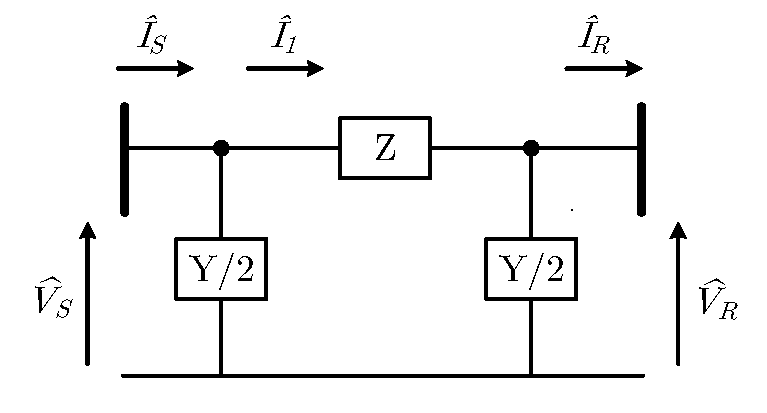
\includegraphics[width=.8\columnwidth]{ModeloLT.pdf}
	%		\caption{Nominal-$\pi$ model of a transmission line.}
	%		\label{fig:ModeloPi}
	%	\end{center}
	%\end{figure}
	\begin{figure}[!t]
		\begin{center}
			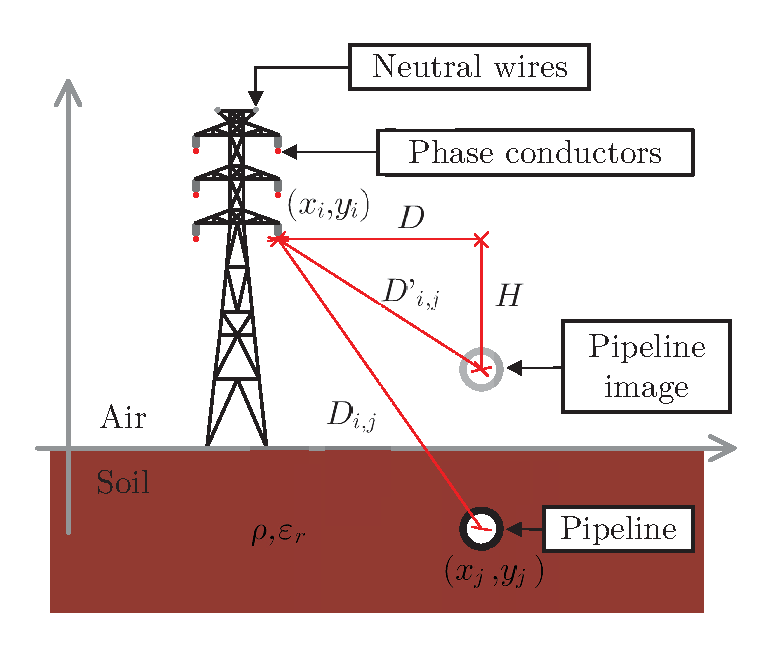
\includegraphics[width=.8\columnwidth]{fig/VistaTorreDuto2.pdf}
			\caption{Phase conductors, neutral wires and pipeline.}
			\label{fig:VistaTorreDuto}
		\end{center}
	\end{figure}
	\begin{figure}[!t]
		\begin{center}
			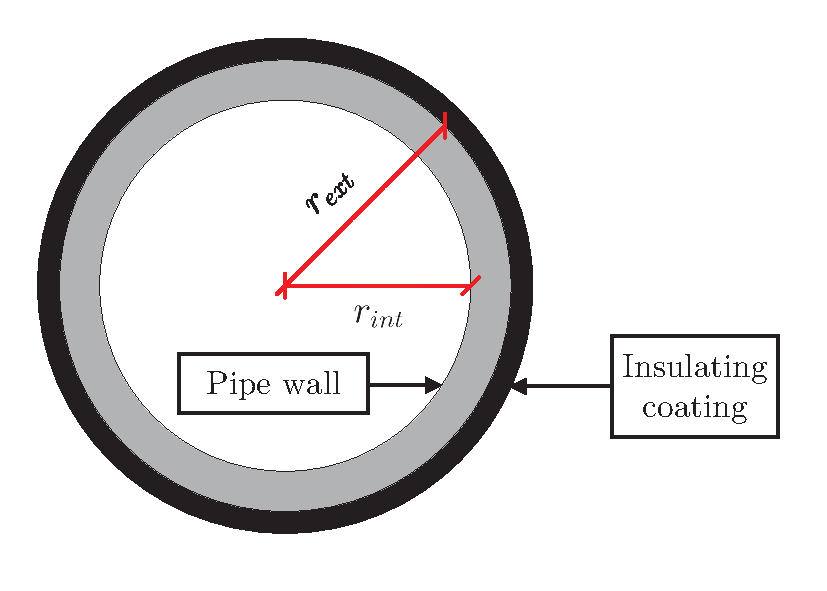
\includegraphics[width=.8\columnwidth]{fig/Pipe2.pdf}
			\caption{Cross section of a pipeline.}
			\label{fig:Pipe}
		\end{center}
	\end{figure}
	\begin{equation}\label{eq:GMR}
		\begin{aligned}
			\ln(GMR_{TU})=&\ln(r_{ext})-\frac{\frac{r_{ext}^4}{4}-r_{ext}^2r_{int}^2}{(r_{ext}^2-r_{int}^2)^2}+ \\
			&\frac{r_{int}^4[\frac{3}{4}+ln(\frac{r_{int}}{r_{int}})]}{(r_{ext}^2-r_{int}^2)^2},
		\end{aligned}
	\end{equation}
	in which $r_{ext}$ and $r_{int}$ express, respectively, the external and the internal radius of the tubular pipeline structure, in meters.
	
	The first term in \eqref{eq:CarsonMutual} and the second term in \eqref{eq:CarsonSelf} correspond to the ground return impedance for a perfectly conductive soil. The improper integrals, known as Carson's integrals, represent the effects of the soil with finite resistivity, including losses caused by current return. The Carson's integral solution has been assessed by several researchers using numerical techniques based on quadratures, power series expansion or deduction of simplified expressions, being worth mentioning the formulas derived by Carson-Clem, Deri, Lucca and Ametani \cite{CIGREWG36,DeriA.Tevan1981,Lucca1994,Ametani2009}. The use of simplified formulas is convenient, but may introduce significant errors if the particularities of the interference problem under study are not well understood. In general, these expressions produce satisfactory results for low frequencies and relatively small spacings between conductors, which imposes a limitation to the calculation model.
	
	In \cite{Theodoulidis2015}, Theodoulidis et al. show that the Carson's integral can be evaluated analytically, with floating-point precision and without convergence problems, by means of a closed-form solution, i.e.  expressed in terms of one or more functions whose behavior is well known. Indeed, the integrals in \eqref{eq:CarsonMutual} and \eqref{eq:CarsonSelf} can be written as \eqref{eq:CarsonAna} with the variable change expressed as shown in \eqref{eq:VarChangeU1} and \eqref{eq:VarChangeU2}:
	%\small
	\begin{equation}\label{eq:CarsonAna}
		\begin{aligned}
			&\int_{0}^{\infty}\frac{2e^{-H\lambda}}{\lambda+\sqrt{\lambda^2+j\frac{\omega\mu_{0}}{\rho}-\omega^2\mu_{0}\varepsilon_{0}\varepsilon_{r}}}\cos\left( \lambda D \right) d\lambda= \\
			&\frac{\pi}{2u_1}[\widehat{H_1}(u_1)\scalebox{0.75}[1.0]{\( - \)}\widehat{Y_1}(u_1)]\scalebox{0.75}[1.0]{\( - \)}\frac{1}{u_1^2}\scalebox{0.75}[1.0]{\( + \)}\frac{\pi}{2u_2}[\widehat{H_1}(u_2)\scalebox{0.75}[1.0]{\( - \)}\widehat{Y_1}(u_2)]\scalebox{0.75}[1.0]{\( - \)}\frac{1}{u_2^2},
		\end{aligned}
	\end{equation}
	%\normalsize
	
	\begin{equation}\label{eq:VarChangeU1}
		\begin{aligned}
			u_1=(H-jD)\sqrt{j\frac{\omega\mu_0}{\rho}-\omega^2\mu_0\varepsilon_0\varepsilon_r},
		\end{aligned}
	\end{equation}
	
	\begin{equation}\label{eq:VarChangeU2}
		\begin{aligned}
			u_2=(H+jD)\sqrt{j\frac{\omega\mu_0}{\rho}-\omega^2\mu_0\varepsilon_0\varepsilon_r},
		\end{aligned}
	\end{equation}
	in which $\widehat{H_1}$ is the Struve function and $\widehat{Y_1}$ is the Bessel function of the second type, both of first order \cite{Theodoulidis2015}.
	
	Since the interfering pipeline is not energized by the power system, it can be handled in the same way as the neutral conductors in the calculation model. Therefore, nodes related to the neutral conductors and the pipeline can be eliminated from \eqref{eq:MatrizImpSerie} using Kron reduction. For a 3-phase system, considering neutral conductors and the pipeline grounded on both extremities, one can write the following equivalent series impedance matrix:
	\begin{equation}\label{eq:MatrizZEq}
		\begin{aligned}
			\mathbf{Z_{EQ}}=\mathbf{Z_{FF}}-\mathbf{Z_{FG}}\cdot\mathbf{Z_{GG}}^{-1}\cdot\mathbf{Z_{GF}},
		\end{aligned}
	\end{equation}
	being:
	\begin{equation}\label{eq:MatrizFF}
		\begin{aligned}
			\arraycolsep=0.8pt % default: 5pt
			\medmuskip = -2mu % default: 4mu plus 2mu minus 4mu
			\def\arraystretch{1.2}
			&\mathbf{Z_{FF}}
			=
			\begin{bmatrix}
				Z_{a,a} & Z_{a,b} & Z_{a,c}  \\
				Z_{b,a} & Z_{b,b} & Z_{b,c} \\
				Z_{c,a} & Z_{c,b} & Z_{c,c} \\
			\end{bmatrix},
		\end{aligned}
	\end{equation}
	\begin{equation}\label{eq:MatrizFG}
		\begin{aligned}
			\arraycolsep=0.8pt % default: 5pt
			\medmuskip = -2mu % default: 4mu plus 2mu minus 4mu
			\def\arraystretch{1.2}
			&\mathbf{Z_{FG}}
			=
			\begin{bmatrix}
				Z_{a,n1} & \ldots & Z_{a,nN} & Z_{a,p}  \\
				Z_{b,n1} & \ldots & Z_{b,nN} & Z_{b,p} \\
				Z_{c,n1} & \ldots & Z_{c,nN} & Z_{c,p} \\
			\end{bmatrix}, 
		\end{aligned}
	\end{equation}
	\begin{equation}\label{eq:MatrizGG}
		\begin{aligned}
			\arraycolsep=0.8pt % default: 5pt
			\medmuskip = -2mu % default: 4mu plus 2mu minus 4mu
			\def\arraystretch{1.2}
			&\mathbf{Z_{GG}}
			=
			\begin{bmatrix}
				Z_{n1,n1} & \ldots & Z_{n1,nN} & Z_{n1,p}  \\
				\vdots & \ddots & \vdots & \vdots \\
				Z_{nN,n1} & \ldots & Z_{nN,nN} & Z_{nN,p} \\
				Z_{p,n1} & \ldots & Z_{p,nN} & Z_{p,p} \\
			\end{bmatrix},
		\end{aligned}
	\end{equation}
	\begin{equation}\label{eq:MatrizGF}
		\begin{aligned}
			\arraycolsep=0.8pt % default: 5pt
			\medmuskip = -2mu % default: 4mu plus 2mu minus 4mu
			\def\arraystretch{1.2}
			&\mathbf{Z_{GF}}
			=
			\begin{bmatrix}
				Z_{n1,a} & \ldots & Z_{nN,a} & Z_{p,a}  \\
				Z_{n1,b} & \ldots & Z_{nN,b} & Z_{p,b} \\
				Z_{n1,c} & \ldots & Z_{nN,c} & Z_{p,c} \\
			\end{bmatrix}.
		\end{aligned} 
	\end{equation}
	
	Assuming the transmission line is transposed, the matrix \eqref{eq:MatrizZEq} is rewritten as:
	\begin{equation}\label{eq:MatrizTransp}
		\begin{aligned}
			\arraycolsep=0.8pt % default: 5pt
			\medmuskip = -2mu % default: 4mu plus 2mu minus 4mu
			\def\arraystretch{1.2}
			&\mathbf{Z_{EQ,T}}
			=
			\begin{bmatrix}
				Z_{P} & Z_{M} & Z_{M}  \\
				Z_{M} & Z_{P} & Z_{M} \\
				Z_{P} & Z_{M} & Z_{P} \\
			\end{bmatrix}.
		\end{aligned} 
	\end{equation}
	in which $Z_{P}$ and $Z_{M}$ are computed using:
	\begin{equation}\label{eq:scalarZP}
		\begin{aligned}
			&Z_{P}=\frac{\mathbf{Z_{EQ}}(1,1)+\mathbf{Z_{EQ}}(2,2)+\mathbf{Z_{EQ}}(3,3)}{3},
		\end{aligned}
	\end{equation}
	\begin{equation}\label{eq:scalarZM}
		\begin{aligned}
			&Z_{M}=\frac{\mathbf{Z_{EQ}}(1,2)+\mathbf{Z_{EQ}}(2,3)+\mathbf{Z_{EQ}}(3,1)}{3}.
		\end{aligned}
	\end{equation}
	
	Finally, the sequence impedance matrix $\mathbf{Z_{012}}$ is obtained by applying the Fortescue transformation\footnote{Equation \eqref{eq:Transform} shows the Fostescue transformation matrix for an ABC system. For ACB systems, the matrix must be adapted.}:
	\begin{equation}\label{eq:MatrizImpSeq}
		\begin{aligned}
			\arraycolsep=0.8pt % default: 5pt
			\medmuskip = -2mu % default: 4mu plus 2mu minus 4mu
			\def\arraystretch{1.2}
			&\mathbf{Z_{012}}
			=\mathbf{T}^{-1}
			\cdot\mathbf{Z_{EQ,T}}\cdot\mathbf{T}=
			\begin{bmatrix}
				Z_0 & 0 & 0  \\
				0 & Z_1 & 0 \\
				0 & 0 & Z_2 \\
			\end{bmatrix},
		\end{aligned} 
	\end{equation}
	being
	\begin{equation}\label{eq:Transform}
		\begin{aligned}
			\arraycolsep=0.8pt % default: 5pt
			\medmuskip = -2mu % default: 4mu plus 2mu minus 4mu
			\def\arraystretch{1.2}
			&\mathbf{T}
			=\frac{1}{3}
			\begin{bmatrix}
				1 & 1 & 1  \\
				1 & a & a^2 \\
				1 & a^2 & a \\
			\end{bmatrix}, \textrm{with}~ a=1\angle 120^\circ,
		\end{aligned} 
	\end{equation}
	in which $Z_0$, $Z_1$ and $Z_2$ are, respectively, the zero, positive and negative sequence impedances of the transmission line, in ohms per unit length.
	
	A similar procedure is performed to determine the transmission line admittances. Referring again to the dimensions shown in Figs. \ref{fig:VistaTorreDuto} and \ref{fig:Pipe}, and using the same notation as in the calculations developed so far, the matrix $\mathbf{P}$ is formed with the Maxwell's potential coefficients defined in \eqref{eq:Pij} and \eqref{eq:Pii}.
	\begin{equation}\label{eq:MatrizAdm}
		\arraycolsep=0.7pt % default: 5pt
		\medmuskip = -1mu % default: 4mu plus 2mu minus 4mu
		\def\arraystretch{.9}
		\mathbf{P}
		=
		\begin{bmatrix}
			P_{a,a} & P_{a,b} & P_{a,c} & P_{a,n1} & \ldots & P_{a,nN} & P_{a,p}  \\
			P_{b,a} & P_{b,b} & P_{b,c} & P_{b,n1} & \ldots & P_{b,nN} & P_{b,p}  \\
			P_{c,a} & P_{c,b} & P_{c,c} & P_{c,n1} & \ldots & P_{c,nN} & P_{c,p}  \\
			\vdots & \vdots & \vdots & \vdots & \ddots & \vdots & \vdots  \\
			P_{nN,a} & P_{nN,b} & P_{nN,c} & P_{nN,n1} & \ldots & P_{nN,nN} & P_{nN,p}  \\
			P_{p,a} & P_{p,b} & P_{p,c} & P_{p,n1} & \ldots & P_{p,nN} & P_{p,p}
		\end{bmatrix}
	\end{equation}
	
	\begin{equation}\label{eq:Pij}
		\begin{aligned}
			P_{i,j}=\frac{1}{2\pi\varepsilon_{0}\varepsilon_{r}}\ln\left(\frac{D_{i,j}'}{D_{i,j}}\right).
		\end{aligned}
	\end{equation}
	\begin{equation}\label{eq:Pii}
		\begin{aligned}
			P_{i,i}=\frac{1}{2\pi\varepsilon_{0}\varepsilon_{r}}\ln\left(\frac{D_{i,i}'}{r_{ext}}\right).
		\end{aligned}
	\end{equation}
	
	By analyzing \eqref{eq:Pij} and \eqref{eq:Pii}, which are valid for the 60 Hz frequency, it is observed that the transmission line shunt admittances are determined, essentially, by the configuration of the aboveground conductors and by the electrical permittivity of the medium. Therefore, no influences of interference with underground metallic pipes are expected, since they are immersed in a conductive medium (the ground), which is outside the electrostatic coupling region. Obviously, if interference occurs with metallic pipes above ground level, the transmission line admittances will be affected. Besides, for a low frequency scenario, Maxwell's potential coefficients are unaffected by the soil resistivity. In this section, further calculation steps of shunt admittances are omitted, since they are similar to those shown in \eqref{eq:MatrizZEq}-\eqref{eq:MatrizImpSeq}.
	
	\subsection{Accounting for the Soil Stratification in the Line Parameters Calculation Model}
	Fig. \ref{fig:VistaTorreDuto} depicts a case where the soil is perfectly uniform, with electrical resistivity $\rho$ for all $y\in(0, \infty)$, which is considered in Carson's equations \eqref{eq:CarsonMutual}-\eqref{eq:CarsonSelf}. However, real soils are more complex structures, composed by solid, liquid and gaseous elements, whose electrical resistivity is dependent on the presence of water, particle porosity, type of electrolyte and temperature \cite{He2012}.
	
	
	In practical situations, the soil electrical resistivity is commonly obtained by the Wenner's method, which consists of taking successive readings of an apparent electrical resistivity value from the surface of the soil in different locations and for several depths \cite{NBR7117}.
	
	The process of deriving a layered soil model from the apparent resistivity measurements is known as soil stratification. Fig. \ref{fig:EstratSolo} shows a real soil with several layers with different resistivities $\rho_i$ and thickness $h_i$, and its corresponding model.
	
	\begin{figure}[!hbt]
		\begin{center}
			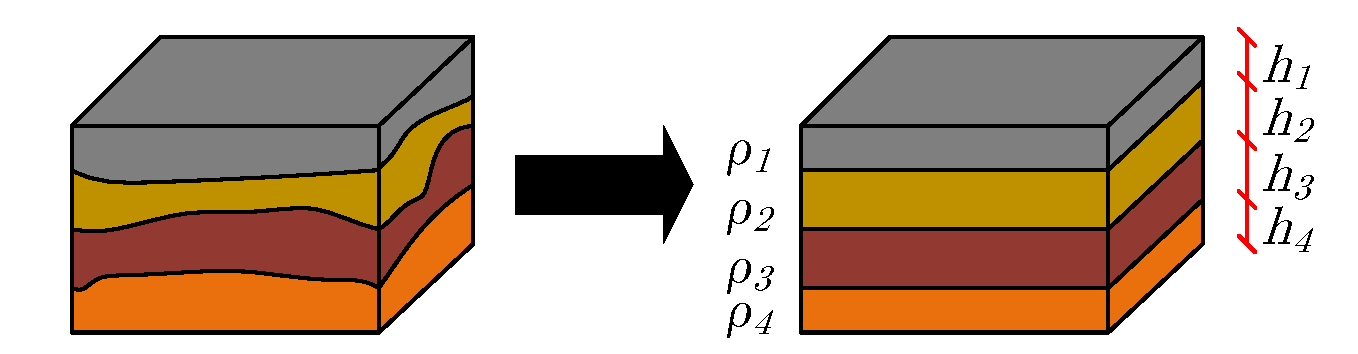
\includegraphics[width=1\columnwidth]{fig/EstratSolo2.pdf}
			\caption{Real soil and stratified model.}
			\label{fig:EstratSolo}
		\end{center}
	\end{figure}
	
	The uniform soil model corresponds to the simple arithmetic mean of the apparent resistivity values. Modeling soils stratified in two or more layers requires more sophisticated numerical methods. The problem of soil stratification is well known in electrical grounding applications \cite{He2012}, as well as the uncertainties inherent to the uniform soil model \cite{IEEEStd80}.
	
	The Finite Element method has been increasingly used in solving problems involving multilayered soils. Although this is a precise approach, it is also computationally expensive. An alternative strategy that has presented valid results in previous studies is to reduce the multilayered model to a uniform equivalent and apply the classic coupling equations such as the Carson's ones \cite{Furlan2015}.
	
	A multi-layered soil, described by $N$ values of resistivity $[\rho_1, \rho_2, \rho_3, ..., \rho_N]$ and $N-1$ thickness values $[h_1, h_2, h_3, ..., h_{(N-1)}]$, can be reduced to a uniform equivalent as described in \cite{Martins-Britto2019}, whose effect is illustrated in Fig. \ref{fig:Hummel}.
	
	\begin{figure}[!hbt]
		\begin{center}
			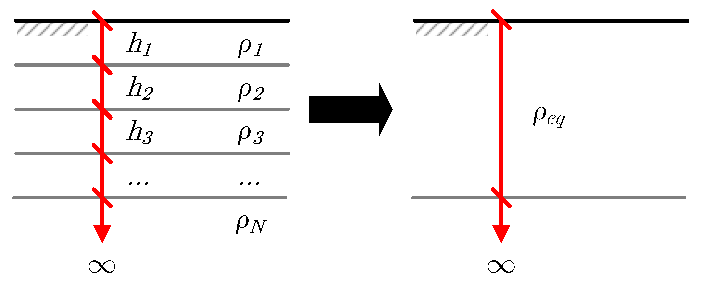
\includegraphics[width=1\columnwidth]{fig/Hummel2.pdf}
			\caption{Stratified soil and its equivalent uniform model.}
			\label{fig:Hummel}
		\end{center}
	\end{figure}
	
	
	
	\begin{figure*}[ht]
		\begin{equation}\label{eq:sigma_recursive_1}
			\sigma_{N-1,N}=\sigma_{N-1} \left[\frac{(\sqrt{\sigma_{N-1}}+\sqrt{\sigma_N})-(\sqrt{\sigma_{N-1}}-\sqrt{\sigma_N})e^{-2h_{N-1}\sqrt{\pi f \mu_{N-1}\sigma_{N-1}}}}{(\sqrt{\sigma_{N-1}}+\sqrt{\sigma_N})+(\sqrt{\sigma_{N-1}}-\sqrt{\sigma_N})e^{-2h_{N-1}\sqrt{\pi f \mu_{N-1}\sigma_{N-1}}}}\right]^2, 
		\end{equation}
		\begin{center}
			$\vdots$
		\end{center}
		\begin{equation}\label{eq:sigma_recursive_2}
			\sigma_{m-1,m}=\sigma_{m-1} \left[\frac{(\sqrt{\sigma_{m-1}}+\sqrt{\sigma_{m-1,m}})-(\sqrt{\sigma_{m-1}}-\sqrt{\sigma_{m-1,m}})e^{-2h_{m-1}\sqrt{\pi f \mu_{m-1}\sigma_{m-1}}}}{(\sqrt{\sigma_{m-1}}+\sqrt{\sigma_{m-1,m}})+(\sqrt{\sigma_{m-1}}-\sqrt{\sigma_{m-1,m}})e^{-2h_{m-1}\sqrt{\pi f \mu_{m-1}\sigma_{m-1}}}}\right]^2,
		\end{equation}
		
		\begin{equation}\label{eq:sigma_recursive_3}
			\sigma_{eq}=\sigma_1 \left[\frac{(\sqrt{\sigma_1}+\sqrt{\sigma_{m-1,m}})-(\sqrt{\sigma_1}-\sqrt{\sigma_{m-1,m}})e^{-2h_1\sqrt{\pi f \mu_1\sigma_1}}}{(\sqrt{\sigma_1}+\sqrt{\sigma_{m-1,m}})+(\sqrt{\sigma_1}-\sqrt{\sigma_{m-1,m}})e^{-2h_1\sqrt{\pi f \mu_1\sigma_1}}}\right]^2, (1\leq m \leq N-2).
		\end{equation}
		
		\hrulefill
	\end{figure*} 
	
	
	Considering $\sigma_{N} = 1/\rho_{N}$  and $f$ being the power system frequency, in hertz, the presence of multiple layers with different constitutive properties is accounted by replacing the uniform variable $\sigma$ in Carson equation by the equivalent parameter $\sigma_{eq}$, defined as in (\ref{eq:sigma_recursive_1})-(\ref{eq:sigma_recursive_3}).
	
	This approach has been proved to provide accurate results yielding a single real-valued parameter that can be readily used with the classic Carson equation (\ref{eq:CarsonMutual}), therefore being fully compatible with the native ATP routines that handle transmission line parameters \cite{Martins-Britto2019}.
	
	
	\section{NUMERICAL RESULTS}
	
	The transmission system is composed of a 200 km long power line sharing the right-of-way with an 8" diameter underground carbon steel pipeline installed at 1.5 m depth, which runs parallel to the transmission line axis along the entire course. Fig.  \ref{fig:SistTesteCorte} shows the geometry of the typical transmission line tower, indicating the distance from the parallel pipeline, with dimensions in meters.
	
	\begin{figure}[hbt]
		\begin{center}
			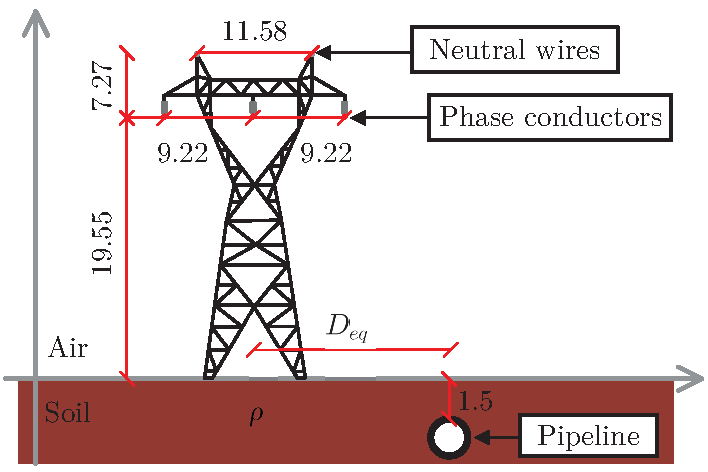
\includegraphics[width=.8\columnwidth]{fig/SistTesteCorte2.pdf}
			\caption{Geometry of the typical tower.}
			\label{fig:SistTesteCorte}
		\end{center}
	\end{figure}
	
	The specifications of the transmission line conductors  are given in Table \ref{table:LTCond}. The pipeline characteristics are provided in Table \ref{table:PipeParam}.
	
	\begin{table}[!hbt]
		\renewcommand{\arraystretch}{1.3}
		\caption{Specifications of transmission line conductors}
		\label{table:LTCond}
		\centering
		\begin{tabular}{|c|c|c|}
			\hline
			\textbf{Conductor} & \textbf{Description} & \textbf{Temperature} \\
			\hline
			Phases & ACSR 636 MCM 27/7 (Peacock) & 50 °C\\
			\hline
			Neutral & Steel 3/8” HS & 50 °C\\
			\hline
		\end{tabular}
	\end{table}
	
	\begin{table}[!hbt]
		\renewcommand{\arraystretch}{1.3}
		\caption{Pipeline characteristics}
		\label{table:PipeParam}
		\centering
		\begin{tabular}{|c|c|}
			\hline
			\textbf{Parameter} & \textbf{Value} \\
			\hline
			Internal radius [m] & 0.1014\\
			\hline
			External radius [m] & 0.1095\\
			\hline
			Electrical resistivity [$\Omega$.m] & $1.72\times10^{-7}$\\
			\hline
			Magnetic permeability [H/m] & $3.77\times10^{-4}$\\
			\hline
		\end{tabular}
	\end{table}
	
	
	%\begin{table}[!hbt]
	%	\renewcommand{\arraystretch}{1.3}
	%	\caption{Pipeline characteristics}
	%	\label{table:PipeParam}
	%	\centering
	%	\begin{tabular}{|c|c|}
	%		\hline
	%		\textbf{Parameter} & \textbf{Value} \\
	%		\hline
	%		Internal radius [m] & 0.1014\\
	%		\hline
	%		External radius [m] & 0.1095\\
	%		\hline
	%		Electrical resistivity [$\Omega$.m] & $1.72\times10^{-7}$\\
	%		\hline
	%		Magnetic permeability [H/m] & $3.77\times10^{-4}$\\
	%		\hline
	%	\end{tabular}
	%\end{table}
	
	%\begin{figure}[hbt]
	%	\begin{center}
	%		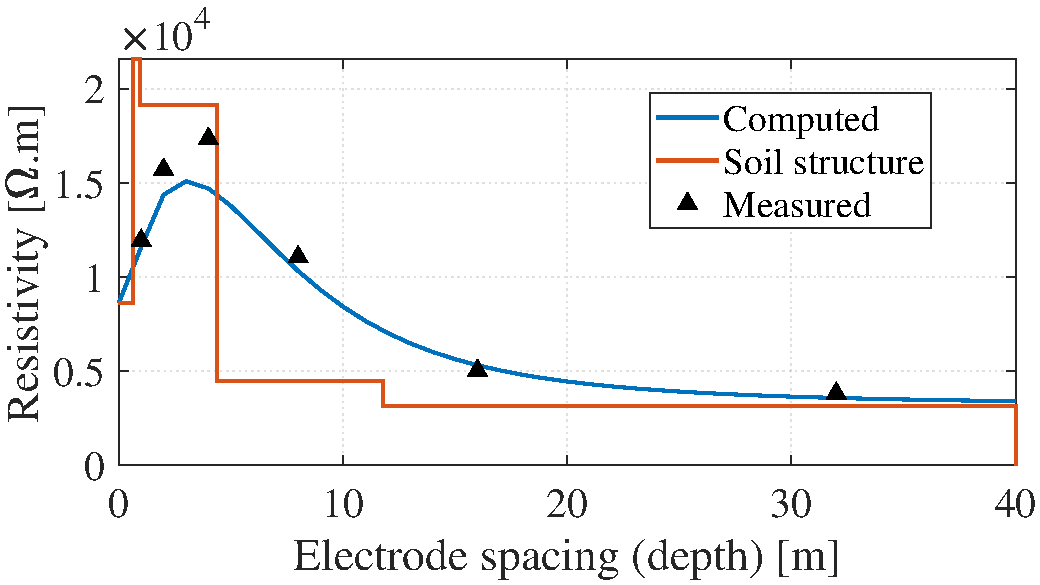
\includegraphics[width=.8\columnwidth]{fig/soilmodel.pdf}
	%		\caption{Five-layered soil model as in \cite{NBR7117}.}
	%		\label{fig:SoilModel}
	%	\end{center}
	%\end{figure}
	
	
	%\begin{table}[!hbt]
	%	\renewcommand{\arraystretch}{1.3}
	%	\caption{Resistivity values from uniform models}
	%	\label{table:ResistivityValues}
	%	\centering
	%	\begin{tabular}{|c|c|}
	%		\hline
	%		\textbf{Model} & \textbf{Resistivity [$\Omega$.m]} \\
	%		\hline
	%		IEEE Std. 80 uniform & 10815\\
	%		\hline
	%		RESAP uniform & 9401.48\\
	%		\hline
	%		Equivalent uniform & 3160.89\\
	%		\hline
	%	\end{tabular}
	%\end{table}
	
	%\begin{table}[!hbt]
	%	\renewcommand{\arraystretch}{1.3}
	%	\centering
	%	\caption{Line parameters of the case study for each scenario}
	%	\begin{tabular}{|c|c|c|}
	%		\hline
	%		\textbf{Cases} & \multicolumn{1}{c|}{\textbf{\boldmath{$Z_{1}$ {[}$\Omega$/m{]}}}} & \multicolumn{1}{c|}{\textbf{\boldmath{$Z_{0}$ {[}$\Omega$/m{]}}}} \\ \hline
	%		1              & 0.1107 + j0.5337                              & 0.5834+j1.8263                                \\ \hline
	%		2              & 0.1107 + j0.5337                              & 0.5775+j1.8146                                \\ \hline
	%		3              & 0.1107 + j0.5337                              & 0.5335+j1.722                                 \\ \hline
	%		4              & 0.1108 + j0.5336                              & 0.3819+j1.3669                                \\ \hline
	%		5              & 0.1108 + j0.5336                              & 0.38+j1.3628                                  \\ \hline
	%		6              & 0.1108 + j0.5336                              & 0.3648+j1.329                                 \\ \hline
	%	\end{tabular}\label{table:LineParam}
	%\end{table}
	
	With the purpose of evaluating the effects of the presence of an interfering structure and the soil influences on line impedances, a parametric study is performed, with separation distances ($D_{eq}$ in Fig. \ref{fig:SistTesteCorte}) varying from 0 to 100 meters, and soil resistivities ranging from 0.01 to 10000 ohms.meter. Fig. \ref{fig:Impedance} presents the zero and positive sequence line impedances in the form of colormaps.
	
	Shunt admittances result in the same values for all scenarios. This is explained by the fact that, in the discussed model, valid for low frequencies, the capacitance is independent of the soil resistivity and that the interfering pipeline is buried beneath the ground, that is, immersed in a conductive medium and, consequently, absent of electrostatic couplings with the energized conductors of the transmission line. It is relevant to note that the positive sequence parameters do not present considerable differences, with an error of less than 1\%. However, the zero sequence impedance is shown to be significantly influenced by interference conditions, in which a discrepancy of 37.5\% is observed between the same resistivity with different interference conditions (0 and 100 meters). 
	
	
	\begin{figure}[hbt]
		\begin{center}
			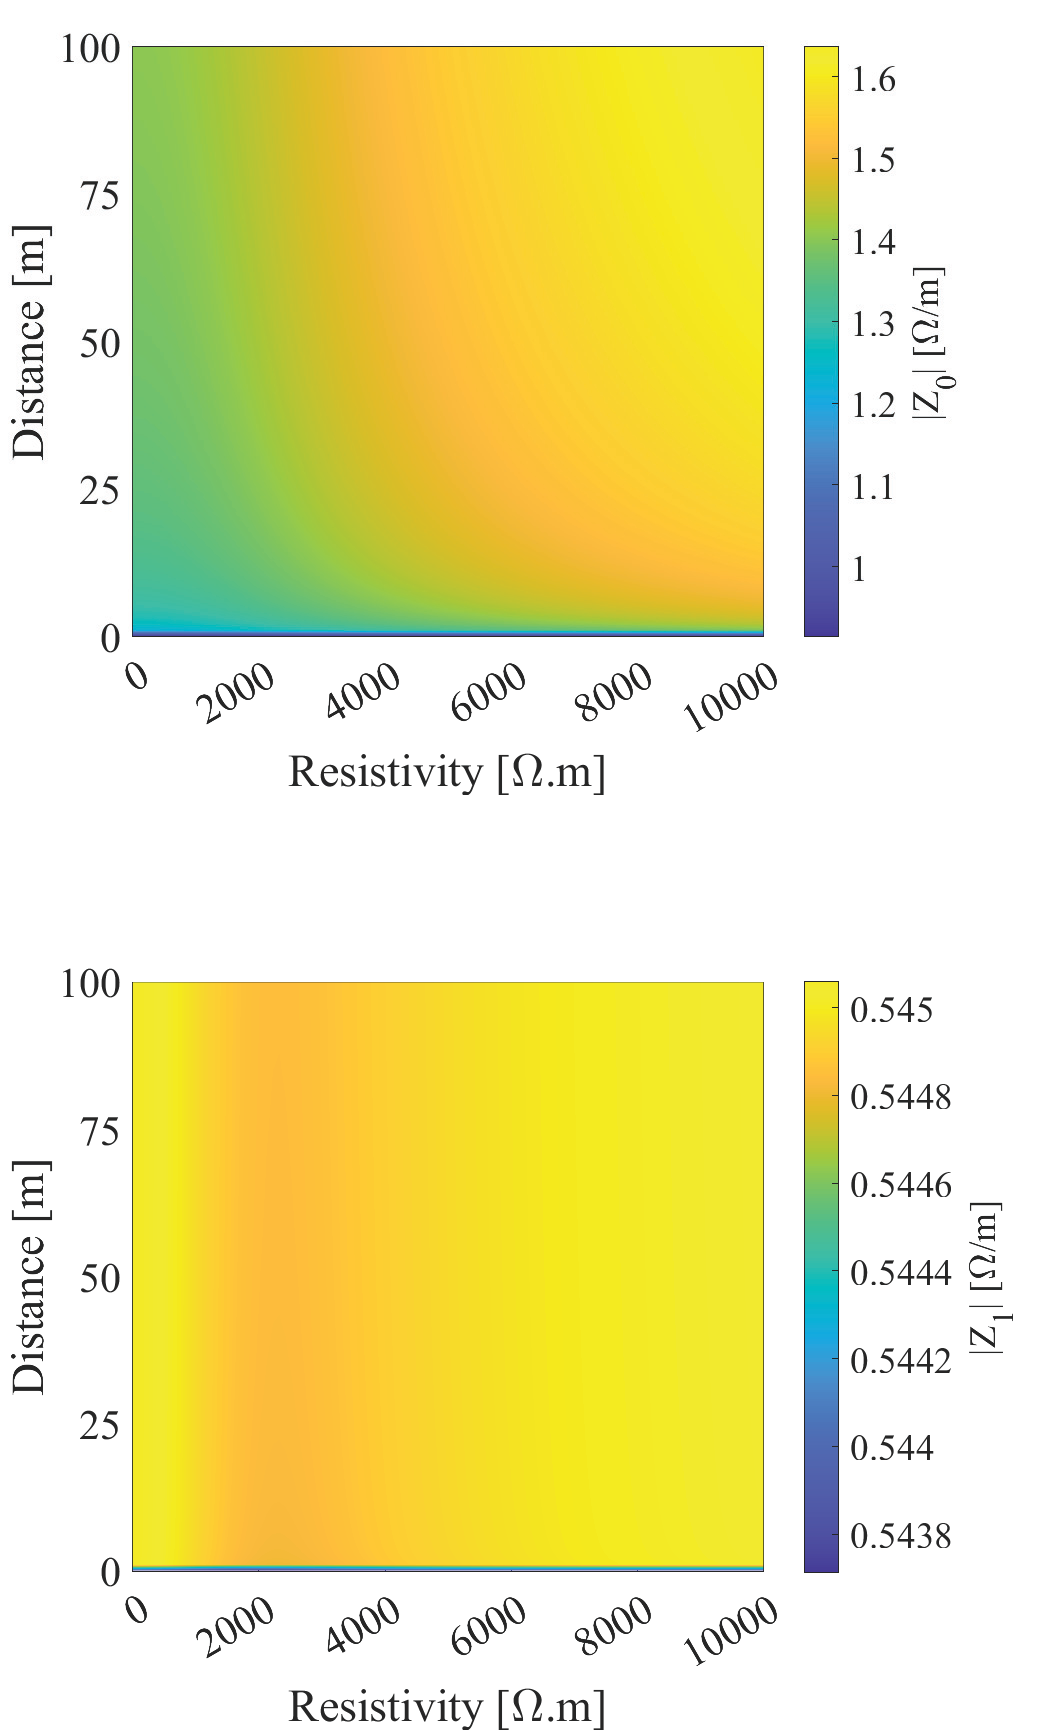
\includegraphics[width=.8\columnwidth]{fig/Impedance2.pdf}
			\caption{Line parameters \textit{versus} resistivity and distance.}
			\label{fig:Impedance}
		\end{center}
	\end{figure}
	
	Fig. \ref{fig:Impedance} indicates that zero sequence impedances are more affected by the presence of an interfering structure than the corresponding positive sequence values. Also, the presence of the pipeline in the vicinities the transmission line seems to more affect its parameters than the soil structure.
	
	\section{CONCLUSIONS}
	
	Results discussed indicate that the zero sequence line parameters are sensitive to the soil model and the presence of interferences, resulting in an error 37.5\% smaller in relation to the extreme distance values (0 and 100 meters), representing distinct conditions of interferences. The positive sequence parameters are not significantly affected by the soil resistivity and the inductive coupling with other installations.
	
	From the above, it is considered of fundamental importance that, in transmission line designs, short-circuit studies, sizing and calibration of protection and fault location devices, precise numerical methods are used to calculate the electrical parameters of power lines. Nevertheless, it is also necessary to ensure the quality of the field gathered information, especially soil resistivity measurements and the survey of interferences with other facilities. 
	
	In the second part of this paper, the effects of transmission line parameters due to interferences and different soil models are further investigated from an engineering application perspective, with numerical analyses 
	of short-circuits and fault location studies on a transmission system.  

	\section*{Acknowledgement}
This work was developed  in partnership with IATI and CEPEL within the scope of the R\&D project PD-06908-0003/2021, sponsored by the Brazilian Agency of Electrical Energy (ANEEL) and EVOLTZ. The authors thank the cooperation of Ms. Larissa Silva (EVOLTZ) and Dr. Marco Antônio M. Rodrigues (CEPEL).
	
	
	\bibliographystyle{IEEEtran}
	\nocite{*}
	\bibliography{refs}
	
	




\end{document}
